\documentclass[article]{jss}

%% -- LaTeX packages and custom commands ---------------------------------------

%% recommended packages
\usepackage{thumbpdf,lmodern}

%% another package (only for this demo article)
\usepackage{framed}

%% new custom commands
\newcommand{\class}[1]{`\code{#1}'}
\newcommand{\fct}[1]{\code{#1()}}

% Custom imports, and defns
\usepackage{booktabs}
\usepackage{amsmath}
\usepackage{amssymb}

\newcommand{\opentsne}{\pkg{openTSNE}}


%% -- Article metainformation (author, title, ...) -----------------------------

%% - \author{} with primary affiliation
%% - \Plainauthor{} without affiliations
%% - Separate authors by \And or \AND (in \author) or by comma (in \Plainauthor).
%% - \AND starts a new line, \And does not.
\author{
  Pavlin G. Poli\v{c}ar\\
  Faculty of Computer and Information Science\\
  University of Ljubljana\\
  Ljubljana, Slovenia
  \AND
  Martin Stra\v{z}ar\\
  Broad Institute of MIT and Harvard\\
  Cambridge, MA, USA
  \AND
  Bla\v{z} Zupan\\
  Faculty of Computer and Information Science\\
  University of Ljubljana\\
  Ljubljana, Slovenia
}
\Plainauthor{P. G. Poli\v{c}ar, M. Stra\v{z}ar, B. Zupan}

%% - \title{} in title case
%% - \Plaintitle{} without LaTeX markup (if any)
%% - \Shorttitle{} with LaTeX markup (if any), used as running title
\title{openTSNE: a modular \proglang{Python} library for t-SNE dimensionality reduction and embedding}
\Plaintitle{openTSNE: a modular Python library for t-SNE dimensionality reduction and embedding}
\Shorttitle{openTSNE: Extensible, parallel implementations of t-SNE}

%% - \Abstract{} almost as usual
\Abstract{
One of the most popular techniques for constructing visualizations of large, high-dimensional data sets is $t$-distributed stochastic neighbor embedding (t-SNE). Recently, several extensions have been proposed to address scalability issues and the quality of the resulting visualizations. We introduce \opentsne, a modular Python library that implements the core t-SNE algorithm and its many extensions. The library is fast and can treat data sets containing millions of data points. We distribute \opentsne\ under the BSD-3-Clause License. Its source code is available at \url{https://github.com/pavlin-policar/openTSNE}.
}

%% - \Keywords{} with LaTeX markup, at least one required
%% - \Plainkeywords{} without LaTeX markup (if necessary)
%% - Should be comma-separated and in sentence case.
\Keywords{t-SNE, embedding, visualization, dimensionality reduction, \proglang{Python}}
\Plainkeywords{t-SNE, embedding, visualization, dimensionality reduction}

%% - \Address{} of at least one author
%% - May contain multiple affiliations for each author
%%   (in extra lines, separated by \emph{and}\\).
%% - May contain multiple authors for the same affiliation
%%   (in the same first line, separated by comma).
\Address{
  Pavlin G. Poli\v{c}ar\\
  Faculty of Computer and Information Science, University of Ljubljana\\
  Ve\v{c}na pot 113, Ljubljana, Slovenia\\
  E-mail: \email{pavlin.policar@fri.uni-lj.si}
}

\begin{document}


%% -- Introduction -------------------------------------------------------------

%% - In principle "as usual".
%% - But should typically have some discussion of both _software_ and _methods_.
%% - Use \proglang{}, \pkg{}, and \code{} markup throughout the manuscript.
%% - If such markup is in (sub)section titles, a plain text version has to be
%%   added as well.
%% - All software mentioned should be properly \cite-d.
%% - All abbreviations should be introduced.
%% - Unless the expansions of abbreviations are proper names (like "Journal
%%   of Statistical Software" above) they should be in sentence case (like
%%   "generalized linear models" below).

\section[Introduction]{Introduction} \label{sec:intro}

The ever-growing volumes of high-dimensional data sets in machine learning call for efficient dimensionality reduction techniques and their implementations, capable of producing informative data visualizations. Popular approaches include principal component analysis, multidimensional scaling, $t$-distributed stochastic neighbor embedding (t-SNE)~\citep{maaten2008visualizing}, and uniform manifold approximation and projections (UMAP)~\citep{2018arXivUMAP}. Among these, t-SNE has received much attention as it can address high volumes of data and reveal the underlying data structure. For instance, t-SNE is widely used in the bioinformatics community in areas such as single-cell transcriptomics~\citep{macosko2015highly,cao2019single,tasic2018shared}, human genetics~\citep{hirata2019genetic}, metagenomic assembly~\citep{beaulaurier2018metagenomic}, the spatial organization of microbial communities~\citep{sheth2019spatial}, and metabolomics~\citep{tkachev2019differences}. To visually explore the data structure, the objects of interest, such as diseased and healthy tissues or single cells, are profiled through thousands of features that include, for example, expression of genes or concentration of metabolites. The task of t-SNE is to embed the objects of interest within a low, preferably two-dimensional embedding. Reports on single-cell gene expression data, our running example, often start with an overview of the cell landscape and use t-SNE to embed high-dimensional expression profiles into a two-dimensional space. Figs.~\ref{fig:macosko}.a and \ref{fig:macosko}.b show two such embeddings.

\begin{figure*}[ht]
  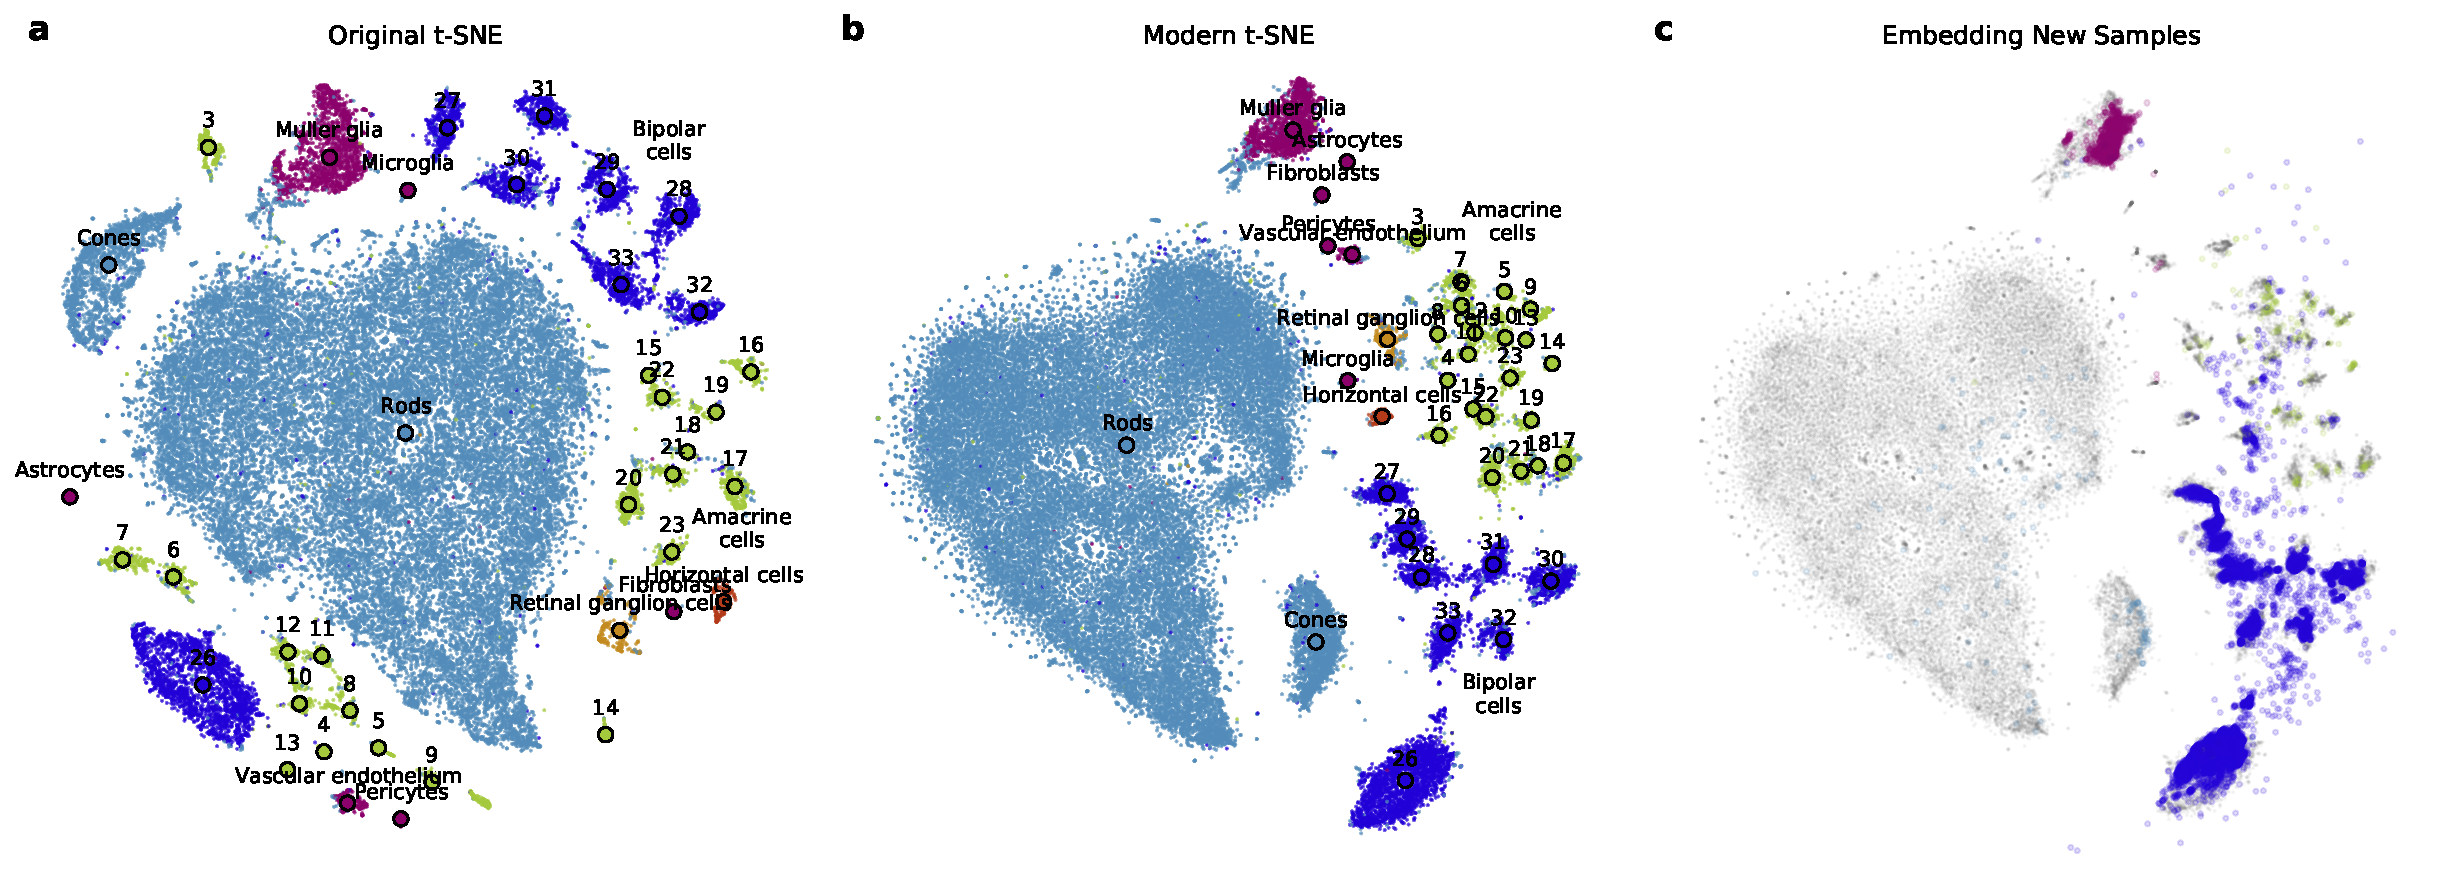
\includegraphics[width=\textwidth]{macosko2015}
  \caption{\label{fig:macosko}
We use \opentsne\ to generate three t-SNE embeddings and demonstrate recent theoretical advances. The data in \textbf{(a)} and \textbf{(b)} includes 44,808 mouse retinal cells (dots in the plots) that are described with high-dimensional gene-expression profiles from \citet{macosko2015highly}. The data in \textbf{(c)} additionally contains 27,499 expression profiles from mouse retinal cells from \citet{shekhar2016comprehensive}. \textbf{(a)} We construct t-SNE embedding following the parameter choices from the original publication by \citet{maaten2008visualizing}. The visualization shows no preservation of the global organization of clusters, resulting from random initialization and an affinity model focused on preserving local neighborhoods. \textbf{(b)} A modern t-SNE embedding, utilizing the latest theoretical advances and practical recommendations constructed using a multi-scale affinity model, preserving both short-range and long-range interactions between data points and initialized so that the global layout is as meaningful as possible. Unlike in \textbf{(a)}, the green and blue clusters representing different sub-types of amacrine and bipolar cells are now localized to the same regions of the space, indicating a higher level of similarity than to other cell types. The embedding in \textbf{(c)} shows how existing t-SNE reference atlases can be used to place new samples into existing embeddings. The positions of new data points correspond to cell types from the reference atlas.
}
\end{figure*}

Despite its utility, t-SNE has often been criticized for its limited scalability, lack of global organization -- t-SNE identifies well-defined clusters that may be arbitrarily scattered throughout the embedding, and the absence of theoretically-founded methods to map new data into existing embeddings~\citep{ding2018interpretable,becht2019dimensionality}. Most of these shortcomings have recently been addressed. \citet{linderman2019fast} developed FIt-SNE, an efficient approximation scheme that massively improves the scalability of t-SNE, achieving linear time complexity in the number of samples. \citet{kobak2019art} proposed several techniques to improve global cluster coherence, including estimating similarities with a mixture of Gaussian kernels. In our previous work, we introduced a principled approach for embedding new samples into existing visualizations~\citep{policar2021embedding}.

However, easy access to efficient implementations almost universally correlates with the widespread adoption of novel computational techniques. Despite the many theoretical advancements, the most popular t-SNE libraries have been slow to incorporate them into their implementations. In this paper, we present \opentsne, our open-source Python implementation of t-SNE, and the recently proposed extensions to t-SNE that \opentsne\ implements. \opentsne\ is easy to install and includes precompiled binaries available through popular Python package managers. It provides a familiar API, making it suitable as a drop-in replacement for existing t-SNE implementations.

%% -- Manuscript ---------------------------------------------------------------

%% - In principle "as usual" again.
%% - When using equations (e.g., {equation}, {eqnarray}, {align}, etc.
%%   avoid empty lines before and after the equation (which would signal a new
%%   paragraph.
%% - When describing longer chunks of code that are _not_ meant for execution
%%   (e.g., a function synopsis or list of arguments), the environment {Code}
%%   is recommended. Alternatively, a plain {verbatim} can also be used.
%%   (For executed code see the next section.)

\section{Methods} \label{sec:methods}

We first introduce the relevant notation and briefly review the core t-SNE
algorithm in Sec.~\ref{sec:meth.tsne}. We then address the criticisms of
scalability (Sec.~\ref{sec:meth.approx}), the ability to add new samples to
existing embeddings (Sec.~\ref{sec:meth.transform}), and improvements that
improve the global consistency of resulting embeddings
(Sec.~\ref{sec:meth.global}).

\subsection{$t$-distributed stochastic neighbor embedding} \label{sec:meth.tsne}

$t$-distributed stochastic neighbor embedding (t-SNE) is a non-linear
dimensionality reduction method that to aims to find a low-dimensional embedding
where neighborhoods are preserved. More formally, given a multi-dimensional data set
$\mathbf{X} = \left \{ \mathbf{x}_1, \mathbf{x}_2, \dots, \mathbf{x}_N \right \}
\in \mathbb{R}^D$ where $N$ is the number of data points in the data set, t-SNE
aims to find a low dimensional embedding $\mathbf{Y} = \left \{ \mathbf{y}_1,
\mathbf{y}_2, \dots, \mathbf{y}_N \right\} \in \mathbb{R}^d$ where $d \ll D$,
such that if points $\mathbf{x}_i$ and $\mathbf{x}_j$ are close in the
high-dimensional space, their corresponding embeddings $\mathbf{y}_i$ and
$\mathbf{y}_j$ are also close. Since t-SNE is primarily used as a visualization
tool, $d$ is typically set to two. The similarity between two data points in the
high-dimensional space is defined using the Gaussian kernel
\begin{equation}
p_{j \mid i} = \frac{\exp \left ( -\frac{1}{2} \mathcal{D}(\mathbf{x}_i, \mathbf{x}_j ) / \sigma_i^2 \right )}
{\sum_{k \neq i } \exp \left ( -\frac{1}{2} \mathcal{D}(\mathbf{x}_i, \mathbf{x}_k ) / \sigma_i^2 \right )}, \quad p_{i \mid i} = 0 \notag
\label{eq:gaussian_kernel}
\end{equation}
where $\mathcal{D}$ is some distance measure. The values $p_{j \mid i}$
are then symmetrized to
\begin{equation}
p_{ij} = \frac{p_{j \mid i} + p_{i \mid j}}{2N}.
\label{eq:symmetrize}
\end{equation}

The bandwidth $\sigma_i$ of each Gaussian kernel is selected such that the perplexity of the distribution matches a user-specified parameter value
\begin{equation}
\text{Perplexity} = 2^{H(P_i)} \notag
\end{equation}
where $H(P_i)$ is the Shannon entropy of $P_i$,
\begin{equation}
H(P_i) = -\sum_i p_{j \mid i} \log_2 (p_{j \mid i}). \notag
\end{equation}
This enables t-SNE to adapt to the varying density of the data in the
multi-dimensional space. The perplexity can be interpreted as the continuous
analogue to the number of nearest neighbors to which the distances will be
preserved. 

The similarity between points $\mathbf{y}_i$ and $\mathbf{y}_j$ in the embedding
space is defined using the $t$-distribution with a single degree of freedom
(Cauchy kernel)
\begin{equation}
q_{ij} = \frac{\left ( 1 + || \mathbf{y}_i - \mathbf{y}_j ||^2 \right )^{-1}}
{\sum_{k \neq l}\left ( 1 + || \mathbf{y}_k - \mathbf{y}_l ||^2 \right )^{-1}},
\quad q_{ii} = 0.
\label{eq:cauchy_kernel}
\end{equation}

We use the Kullback-Leibler (KL) divergence to measure the agreement
between the two distributions $\mathbf{P}$ and $\mathbf{Q}$
\begin{equation}
C = \text{KL}(\mathbf{P} \mid \mid \mathbf{Q}) = \sum_{ij} p_{ij} \log \frac{p_{ij}}{q_{ij}}.
\label{eq:kl_divergence}
\end{equation}
The objective is to find embeddings $\mathbf{Y}$ that minimize the KL divergence. The corresponding gradient takes the form
\begin{equation}
\frac{\partial C}{\partial \mathbf{y}_i} = 4 \sum_{j \neq i} \left ( p_{ij} - q_{ij} \right ) \left ( \mathbf{y}_i - \mathbf{y}_j \right ) w_{ij},
\label{eq:tsne_gradient}
\end{equation}
where $w_{ij} = \left ( 1 + || \mathbf{y}_i - \mathbf{y}_j || ^2 \right )^{-1}$
and represents the unnormalized $q_{ij}$.

Optimization is performed using batch gradient descent using the delta-bar-delta update rule~\citep{jacobs1988increased}. The t-SNE optimization procedure consists of two phases: in the first \textit{early exaggeration} phase, the attractive forces between data points are increased by some factor $\rho$, typically set to $12$, so that points in the embedding can more easily move throughout the space and settle near their respective neighbors. In the second phase of the optimization, the attractive forces are then reverted to their original values with $\rho=1$.

\citet{belkina2019automated} later found that convergence can be sped up by
increasing the learning rate from the standard $\eta=200$ to $\eta=N/12$. As a
side-effect, embeddings converge faster, and the number of iterations can be
lowered from the typical 1000 to 750, decreasing the overall runtime.  Modern
t-SNE implementations, including \pkg{FIt-SNE} and \opentsne, have adopted this
convention.

\subsection{Efficient Approximation Schemes} \label{sec:meth.approx}

A direct evaluation of t-SNE gradients requires $\mathcal{O}(N^2)$ operations,
which makes its application impractical to any reasonably-sized data set and
highlights the need for the development of efficient approximation schemes.
\citet{van2014accelerating} observed that the t-SNE gradient can be cast as an
N-body problem where data points represent particles that attract and repel each
other. The gradient from Eqn.~(\ref{eq:tsne_gradient}) can be rewritten as
\begin{equation}
\frac{\partial C}{\partial \mathbf{y}_i} = 4 \Bigg [
\underbrace{\sum_{j \neq i} p_{ij} q_{ij} Z \left ( \mathbf{y}_i - \mathbf{y}_j \right )}_{\text{attractive forces}}  -
\underbrace{\sum_{j \neq i} q_{ij}^2 Z \left ( \mathbf{y}_i - \mathbf{y}_j \right )}_{\text{repulsive forces}}
\Bigg ], \label{eq:grad_attr_rep} \notag
\end{equation}
where $Z = \sum_{k \neq l}\left ( 1 + || \mathbf{y}_k - \mathbf{y}_l ||^2 \right
)^{-1}$. We can view this equation as a particle simulation, where the
two terms represent the attractive and repulsive forces between individual
particles. Each term lends itself to efficient approximations, enabling us to
reduce the time complexity of t-SNE to $\mathcal{O}(N)$. This allows modern
t-SNE implementations to be leveraged for the visualization of data sets
containing up to millions of data points.

\subsubsection*{Attractive Forces}
\citet{van2014accelerating} observed that evaluating the attractive forces
between all pairs of data points is excessive, and that considering only a
handful of nearest neighbors at each point are sufficient to obtain a good
approximation. Therefore, instead of calculating all pairwise interactions, it
is sufficient to only find and evaluate the attraction to a certain number of
$k$ nearest neighbors. Using tree-based nearest-neighbor search methods,
\citet{van2014accelerating} reduced the time complexity to $\mathcal{O}(N \log
N)$. \citet{linderman2019fast} further realized that, qualitatively, embeddings
are visually indistinguishable when using only \textit{approximate} nearest
neighbors, further reducing time complexity to $\mathcal{O}(N)$.

\subsubsection*{Repulsive Forces}
Similarly, the repulsive term can also be approximated, motivated by methods from
particle simulations. \citet{van2014accelerating} proposed an approach based on
N-body simulations and used a space-partitioning Barnes-Hut tree approach to
approximate the interaction between data points. This reduces the time
complexity from $\mathcal{O}(N^2)$ to $\mathcal{O}(N \log N)$. More recently,
\citet{linderman2019fast} proposed an alternative approach, FIt-SNE, based on
non-uniform convolutions which further reduces the time complexity to
$\mathcal{O}(N)$.


\subsection{Embedding New Samples} \label{sec:meth.transform}

t-SNE is non-parametric and does not define an explicit mapping from the
high-dimensional space to the embedding space. Therefore embeddings of new data
points need to be found through the use of optimization
techniques~\citep{policar2021embedding}. When adding new data points to an
existing, reference embedding, the reference data points are fixed in place
while new data points are allowed to find their respective positions. The
optimization remains the same as in standard t-SNE with only slight
modifications to $p_{ij}$ and $q_{ij}$
\begin{align}
p_{j \mid i} = \frac{\exp \left ( -\frac{1}{2} \mathcal{D}(\mathbf{x}_i, \mathbf{v}_j) /  \sigma_i^2 \right )}{\sum_{i} \exp \left ( -\frac{1}{2} \mathcal{D}(\mathbf{x}_i, \mathbf{v}_j) / \sigma_i^2 \right )}, \qquad
q_{j \mid i} = \frac{\left ( 1 + || \mathbf{y}_i - \mathbf{w}_j ||^2 \right )^{-1}}{\sum_{i}\left ( 1 + || \mathbf{y}_i - \mathbf{w}_j ||^2 \right )^{-1}}, \notag
\end{align}
\noindent where $\mathbf{V} = \left \{ \mathbf{v}_1, \mathbf{v}_2, \dots,
\mathbf{v}_M \right \} \in \mathbb{R}^D$ where $M$ is the number of samples in
the new data set and $\mathbf{W} = \left \{ \mathbf{w}_1, \mathbf{w}_2, \dots,
\mathbf{w}_M \right \} \in \mathbb{R}^d$. Additionally, we omit the
symmetrization step in Eqn.~(\ref{eq:symmetrize}). Plugging these terms into
Eqn.~(\ref{eq:kl_divergence}), we obtain the following gradient
\begin{equation}
\frac{\partial C}{\partial \mathbf{w}_j} = 2 \sum_i \left ( p_{j \mid i} - q_{j \mid i} \right ) \left ( \mathbf{y}_i - \mathbf{w}_j \right ) \left ( 1 + || \mathbf{y}_i - \mathbf{w}_j || ^2 \right )^{-1}. \notag
\label{eq:gradient}
\end{equation}

Similarly to standard t-SNE, a direct calculation of gradients takes
$\mathcal{O}(N \cdot M)$ time, but it is straightforward to adapt the Barnes-Hut
and FIt-SNE approximation schemes, reducing the time complexity to
$\mathcal{O}(M \log N)$ and $\mathcal{O}(M)$, respectively. Special care must be
taken to tune the learning rate during optimization as the default values
$\eta=200$ and $\eta=N/12$ result in highly unstable optimization.


\subsection{Improving the Global Structure of Embeddings} \label{sec:meth.global}

One of t-SNE's criticisms is that it fails to preserve long-range distances but instead focuses on capturing the local structure of the data manifold~\citep{becht2019dimensionality}. Recently, several approaches have been proposed to improve the global organization of the resulting embeddings.

\citet{kobak2019umap} showed that the initialization of force-directed layout algorithms, such as t-SNE, UMAP~\citep{2018arXivUMAP}, and ForceAtlas2~\citep{jacomy2014forceatlas2}, largely dictates the global consistency of resulting embeddings. When initialized randomly, clusters are often arbitrarily scattered in the embedding space. However, when using initialization schemes based on PCA or spectral embeddings, the clusters identified in the resulting embedding are typically grouped in a globally coherent manner.

In standard t-SNE, distances between data points are converted to similarities through the use of Gaussian kernels. The perplexity of these kernels governs the sizes of the local neighborhoods which are to be preserved. One easy way to improve the global consistency of resulting embeddings is to increase the sizes of these neighborhoods. This can be achieved by increasing the perplexity parameter. However, this often comes at the price of local structure. \citet{kobak2019art} propose to use mixtures of Gaussians instead to preserve better short-range and long-range distances and, thus, achieve a better trade-off between local and global structure.

Embeddings produced by standard t-SNE often use all available space and separate clusters by only thin boundaries. When working with large data sets, this often obscures the global relationships between clusters as all neighboring groups appear equidistant from one another.  Other dimensionality reduction methods, such as UMAP and ForceAtlas2, produce embeddings where clusters appear more compact, and the white space separating the clusters may be interpreted as a loose measure of distance. Recently, \citet{bohm2020unifying} showed that the exaggeration factor $\rho$ could be used to produce layouts more similar to UMAP and ForceAtlas2. By incorporating exaggeration into later phases of the optimization, t-SNE introduces white space between clusters, which better reflects the global relations between clusters.

Standard t-SNE reveals the clustering structure at a single level of resolution. While the perplexity parameter can be used to control the trade-off between local and global structure, this can be time-consuming, and small, well-defined clusters can be missed. Alternatively, \citet{kobak2019heavy} suggest that varying the degrees of freedom in the $t$-distribution can be used to explore the clustering structure at different levels of resolution. Modifying Eqn.~(\ref{eq:cauchy_kernel}) to $q_{ij} \propto \left ( 1 + || \mathbf{y}_i - \mathbf{y}_j ||^2 / \alpha \right )^{-\alpha}$ allows us to use heavier-tailed distributions to model distances in the embedding space, which acts to highlight small subgroups in the resulting visualization.


\section{Implementation} \label{sec:implementation}

We introduce \opentsne, a comprehensive Python library that implements t-SNE and its numerous recently proposed extensions, including the implementation of efficient approximation schemes allowing the embedding of millions of data points~\citep{van2014accelerating,linderman2019fast}, the addition of new data points into existing embeddings~\citep{policar2019embedding}, various initialization improvements~\citep{kobak2019umap}, extensions~\citep{kobak2019heavy,kobak2019art}, and improved parameter defaults~\citep{belkina2019automated}. When combined, these improvements result in the faster generation of more informative visualizations.

\opentsne\ is compatible with the Python data science ecosystem (e.g. \pkg{numpy}, \pkg{scikit-learn}, \pkg{scanpy}), providing a familiar and intuitive API to users. Its modular design encourages extensibility and experimentation with various parameter settings and changes to the analysis pipeline. \opentsne\ aims to make the latest theoretical advances in t-SNE accessible to the wider data science community. These features are easily accessible through an intuitive API, which closely follows the style \pkg{scikit-learn}~\citep{sklearn_api}, a popular and widely used toolkit for machine learning. The following snippet exemplifies this interface and demonstrates how \opentsne\ can be used to quickly generate several visualizations, each highlighting different aspects of the underlying data structure.
\begin{CodeChunk}
\begin{CodeInput}
from openTSNE import TSNE

# Vanilla t-SNE
tsne_standard = TSNE().fit(x)

# Adapt parameters to better highlight small clusters in the data
tsne_extensions = TSNE(perplexity=50, exaggeration=2, dof=0.8).fit(x)

# Use multiscale kernel for better local/global structure trade-off
from openTSNE.affinity import Multiscale

affinities = Multiscale(x, perplexities=[50, 500])
tsne_multiscale = TSNE().fit(x, affinities=affinites)

# Use the generated embeddings to add new data points
new_embedding = tsne_extensions.transform(x_new)
\end{CodeInput}
\end{CodeChunk}
The code snippet considers a \pkg{numpy} array or \pkg{scipy} sparse matrix \texttt{x} and creates three \texttt{TSNEEmbedding} objects. These represent fully-optimized t-SNE embeddings, and \opentsne\ internally stores them as \pkg{numpy} arrays. These can be manipulated and visualized using standard Python tools. We then select one of these embeddings and use it to embed new data points from \texttt{x\_new} into the embedding space while keeping the reference embedding fixed. Additionally, \opentsne\ provides a more advanced interface that enables the user to change every aspect of the t-SNE optimization procedure. We describe this interface in detail in the \opentsne's on-line documentation.


\section{Summary and discussion} \label{sec:summary}

\subsection{Uncovering Structure in High-Dimensional Data}

Dimensionality reduction techniques implicitly assume that high-dimensional data lies on a lower-dimensional manifold, which a small number of dimensions can accurately capture. However, there is no evidence that every data set can accurately be described using only two dimensions, and any such embedding will inevitably lead to a loss of information. Thus, it is beneficial to examine multiple embeddings, each of which provides a different perspective on topology and other data characteristics.

\begin{figure*}[htbp]
  \center
  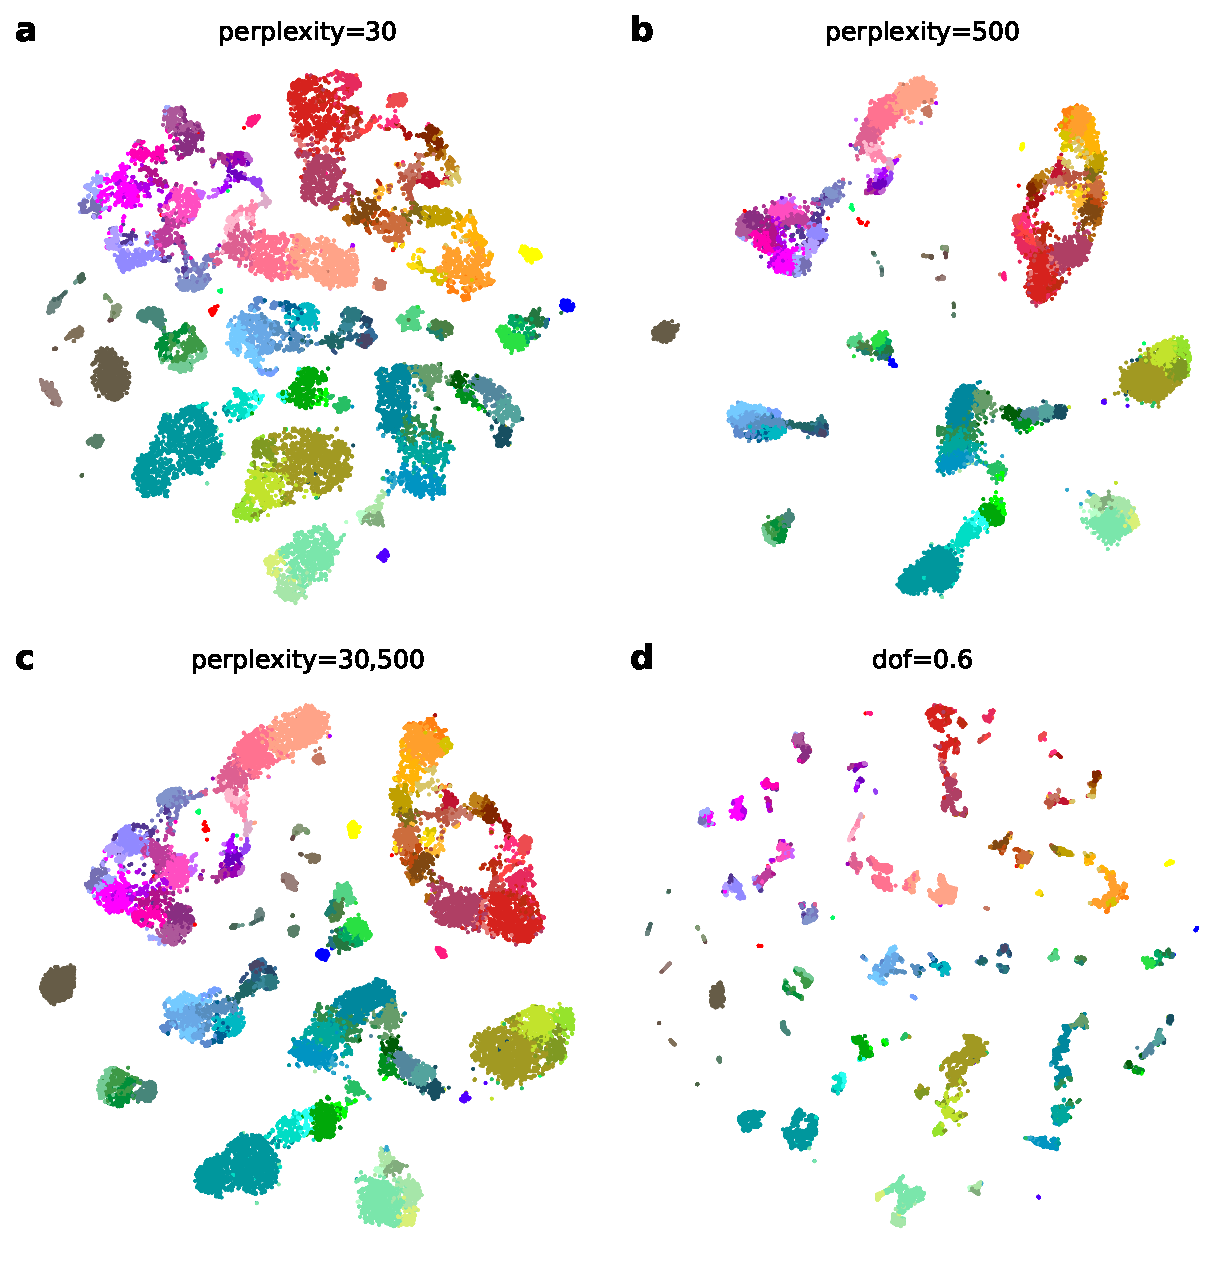
\includegraphics[width=0.75\textwidth]{tasic2018}
  \caption{\label{fig:tasic}
  We use \opentsne\ to create four different
  visualizations of the \citet{tasic2018shared} data,
  each providing a different perspective into the topology of the data.
  The data set contains 21,874 single-cells originating from the mouse
  neocortex. Cluster annotations and colors are taken from the original
  publication. Warm colors correspond to excitatory neurons, cool colors
  correspond to inhibitory neurons, and gray/brown colors correspond to
  non-neuronal cells. Standard t-SNE \textbf{(a)} emphasizes local
  structure while increasing perplexity \textbf{(b)} results in a more
  meaningful layout of the clusters. We can also combine the two
  perplexities by using a multi-scale kernel affinity model \textbf{(c)}
  and obtain a trade-off between global and local structure.
  Alternatively, we can inspect more fine-grained structure and reveal
  smaller clusters by using a more heavy-tailed kernel \textbf{(d)}.}
\end{figure*}

We illustrate this point by generating four different embeddings of the data on single-cell gene expression in mouse brain~\citep{tasic2018shared}. Fig.~\ref{fig:tasic}.a shows an embedding using default t-SNE parameters. While different clusters of excitatory and inhibitory neurons appear close to one another, all clusters appear equidistant from their neighbors, and the overall relations between groups are not obvious. The embedding in Fig.~\ref{fig:tasic}.b focuses on preserving larger neighborhoods of points, resulting in a more globally consistent layout where relations between clusters become more apparent. Here, it is evident from the increased white space between groups that there is one large class of excitatory neurons and two related classes of inhibitory neurons. Unfortunately, focusing on preserving large neighborhoods leads to the absorption of smaller clusters into larger ones. Alternatively, Fig.~\ref{fig:tasic}.c uses multi-scale similarity kernels that aim to preserve both the global organization of clusters and prevent smaller cluster absorption. We constructed the embedding from Fig.~\ref{fig:tasic}.d with the settings used for Fig.~\ref{fig:tasic}.a, but at a finer level of resolution. The figure demonstrates that some clusters are composed of numerous, smaller subgroups representing different cell subpopulations that are not visible under standard parameter settings.

When dealing with data containing millions of data points, standard t-SNE embeddings often become unwieldy -- cluster boundaries are blurred, large clusters absorb smaller ones, and relationships between clusters become increasingly difficult to interpret. We constructed Fig.~\ref{fig:cao}.a from the data containing expression profiles of over two million single cells captured at different time points in mouse development. The embedding indicates numerous clusters with transitions between time points, as marked by the color-coding, that are difficult to interpret. Kobak \& Berens observed that increasing attractive forces between similar data points controlled via the \textit{exaggeration} parameter leads to more compact clusters, and subsequently, more informative visualizations~\citep{kobak2019art}. For instance, \ref{fig:cao}.b doubles the default exaggeration, which uncovers some of the data's overall structure. Further doubling the exaggeration in \ref{fig:cao}.c allows us to observe that the data is comprised of two main groups of cells and eight somewhat smaller clusters. The visualization also reveals several tiny clusters, possibly corresponding to rare cell types.

\begin{figure*}[htbp]
  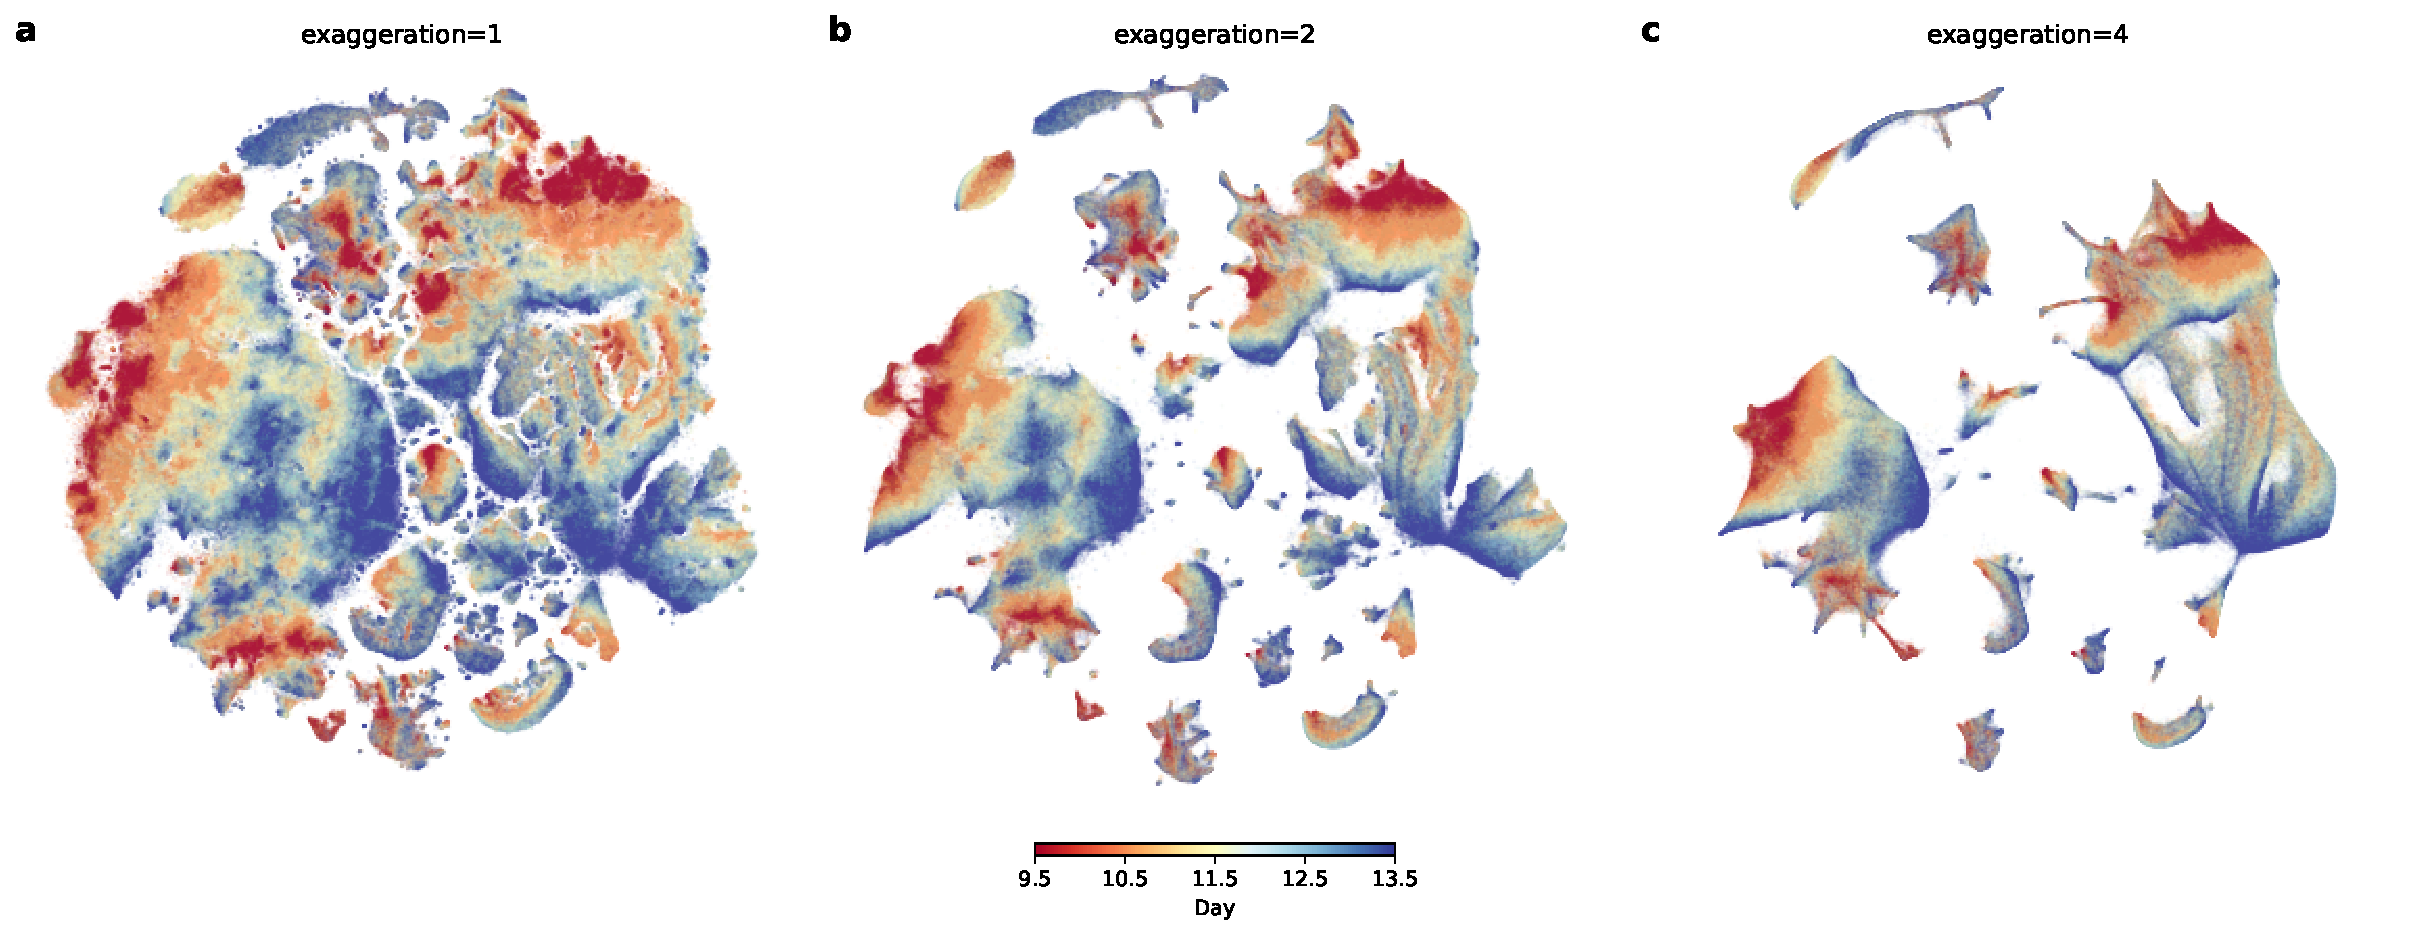
\includegraphics[width=\textwidth]{cao2019}
  \caption{\label{fig:cao}
  Increasing the exaggeration parameter leads to compact clusters, highlighting
  the data's global organization and emphasizing the continuous nature of
  cell state transitions. The data set from \citet{cao2019single}
  contains expression profiles from 2,058,652 single cells. The data were
  collected from mice embryos at different developmental stages at daily
  intervals after 9.5 to 13.5 days. \textbf{(c)} reveals that the data is
  comprised of two main components -- the neural tube and mesenchymal
  cells -- as well as several other smaller clusters. The
  colors indicate developmental progression with red indicating
  least-developed cells and blue indicating most developed cells. The
  overall developmental trajectory is most apparent with higher
  exaggeration levels, showing red cells slowly transitioning into blue
  cells. Progressively easing the exaggeration factor uncovers finer
  clusters within the larger groups, as shown in \textbf{(b)} with
  exaggeration of two and subsequently in \textbf{(a)}, where we show the
  standard t-SNE with no exaggeration. 32,011 putative doublets are
  excluded from the visualizations.
}
\end{figure*}

Exaggeration can highlight transitions between cell states in developmental
studies. Standard t-SNE often produces embeddings with clearly defined, discrete
clusters. We can adjust the level of granularity and resolution of the clusters
with several parameters in Fig.~\ref{fig:tasic}. However, discrete clusters are
often undesired in developmental studies where cells' state is assumed to follow
a continuous transition path. To this end, other embedding techniques such as
UMAP and ForceAtlas2 are used to better capture the continuity between cell
states. Recently, \citet{bohm2020unifying} showed that
embeddings produced by t-SNE with exaggeration values of 4 and $\sim30$
construct embeddings which are markedly similar to UMAP and ForceAtlas2,
respectively. For example, in Fig.~\ref{fig:cao}.a, the developmental trajectory
between different time points is difficult to observe due to many sprawled out
clusters. On the other hand, it is easier to trace the development when we
increase the exaggeration factor from $1$ to $2$ to $4$ in
Figs.~\ref{fig:cao}.b-c.

\subsection{Embedding New Samples}

Unlike other popular dimensionality reduction techniques such as principal
component analysis or autoencoders, t-SNE is a non-parametric method and does
not define an explicit mapping to the embedding space. Therefore, embeddings of
new data points need to be found through
optimization~\citep{policar2021embedding}. \opentsne\ is currently the only
publicly available library allowing users to add new samples to existing
embeddings in a principled manner.

Figs.~\ref{fig:macosko}.b and \ref{fig:macosko}.c demonstrate how we can use a
previously labeled single-cell data set and embed cells from a separate
experiment into the reference landscape. The reference data from
\citet{macosko2015highly} contains gene expression
profiles from mouse retinal cells. By embedding the samples from a similar
experiment on bipolar retinal cells by \citet{shekhar2016comprehensive}, we can correctly map the bipolar cell
clusters onto the reference embedding.

Embedding single cells into existing reference atlases can also be useful for
cell-type classification in cases of unknown cell identities. For instance, in
Fig.~\ref{fig:transform}, we construct a reference embedding using labeled data
from \citet{hochgerner2018conserved} containing
gene-expression profiles of cells from the mouse brain. The authors assign a
type to each cell. We can verify their classification accuracy by visualizing
the expression of well-established gene markers for the major cell types. We
then embed cells from \citet{harris2018classes} into the
constructed cell atlas. In \citet{harris2018classes}, labels are provided only for
neuronal cells. In the resulting mapping, we can quickly identify other
non-neuronal cell types, including oligodendrocytes and astrocytes. We can
further use marker genes to validate that the mapping in the reference landscape
is correct. 

\begin{figure*}[htbp]
  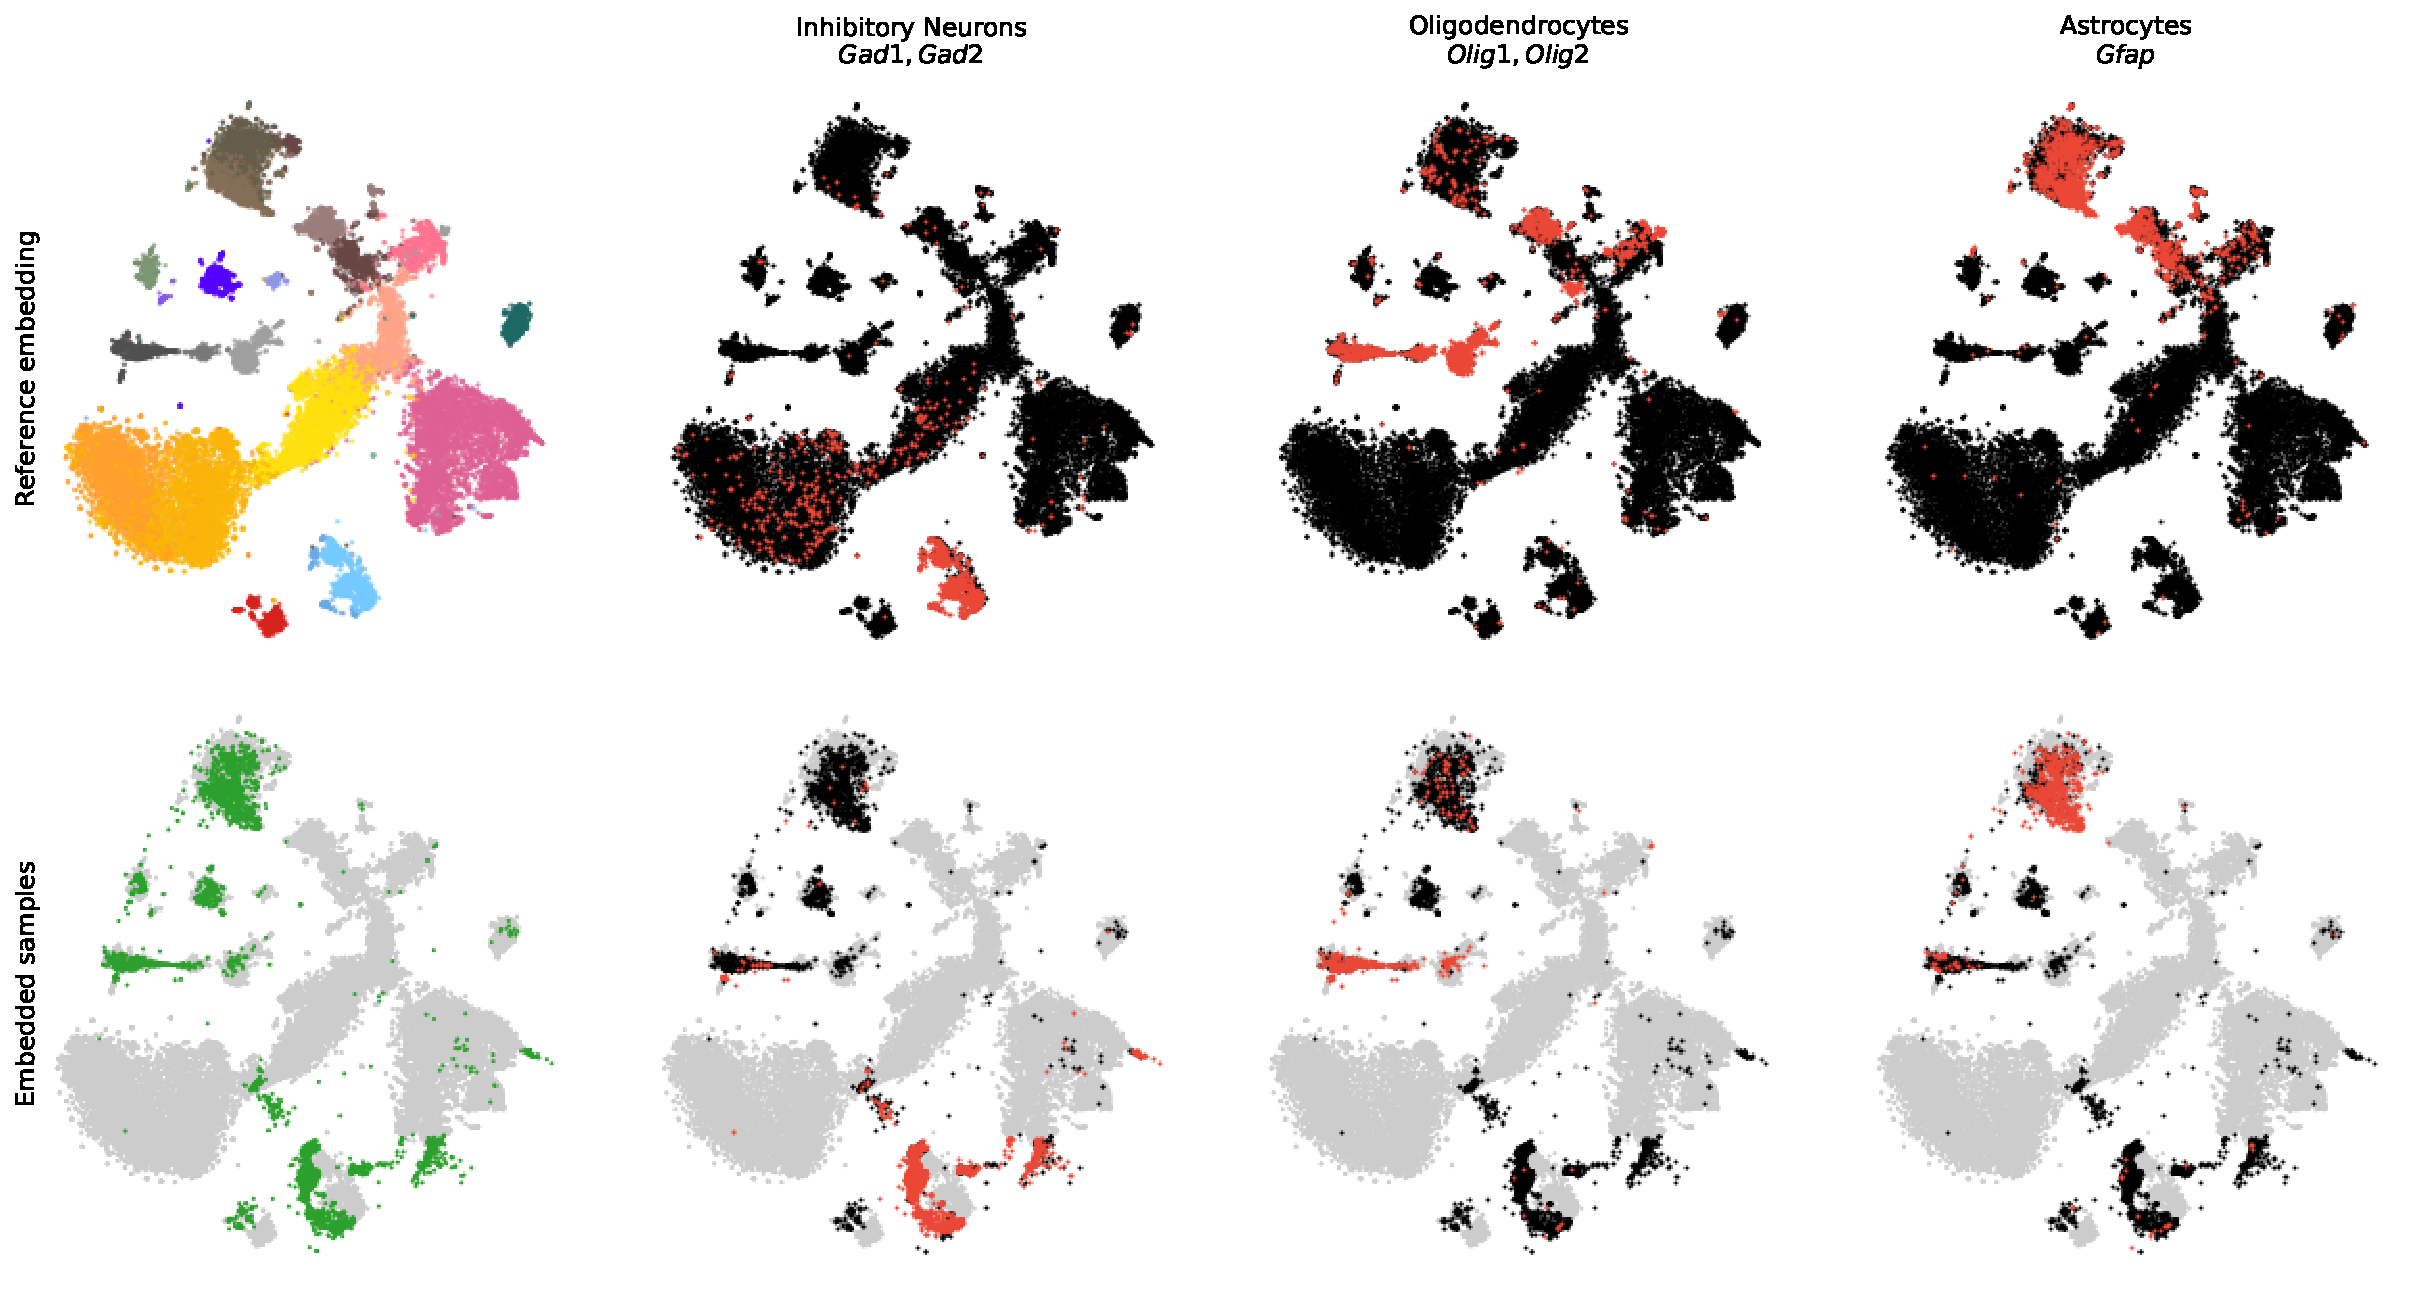
\includegraphics[width=\textwidth]{transform_hochgerner}
  \caption{\label{fig:transform}
  \opentsne\ supports embedding new samples into an existing reference t-SNE
  landscape. For the series of visualizations shown in this figure, we
  first construct a t-SNE embedding for the data from 
  \citet{hochgerner2018conserved} containing 24,185
  developing, single cells from the mouse hippocampus. The data contains
  gene expression in different neurons, supporting glia, and other
  vascular cells (upper left). Data points representing cells are colored
  according to cell-types assigned in the original publication; see the
  legend from Fig.~\ref{fig:tasic} to map colors to cell-type. We then
  embed new, hippocampal cells collected in a study by
  \citet{harris2018classes} using the embedding of \citet{hochgerner2018conserved}
  data as a reference. In their study, \citet{harris2018classes}
  collected 6,971 single-cells and focused on identifying different
  types of inhibitory neurons. However, almost half of the collected cells
  are not neurons and were left uncharacterized. Inspecting the embeddings
  of these cells in the reference embedding (bottom left) reveals that in
  addition to inhibitory neurons, the data contains several supporting
  glial cells as well as a small population of endothelial cells. We can
  verify our approach's accuracy by inspecting marker genes for the major
  cell types in the reference (top row) and embedded samples (bottom row).
}
\end{figure*}

The examples presented above demonstrate how to use \opentsne\ to quickly gain
insight into newly-sequenced, single-cell data sets by utilizing existing cell
atlases. The approach is general and not limited to single-cell gene expression,
and one can, in principle, apply it to any tabular data set regardless of field.

\subsection{Versatility}

Versatility, the ability to use and combine different optimization approaches to
construct different embedding spaces, is another of \opentsne's core design
principles. \citet{kobak2019art} recently provided several recommendations and
tricks to obtain better and more meaningful t-SNE visualizations. These include
multi-scale similarity kernels, perplexity annealing, and increasing
exaggeration when working with massive data sets. \opentsne\ provides a flexible
API to incorporate these improvements in just a few lines of code. Furthermore,
\opentsne\ supports custom affinity models, enabling users to construct t-SNE
embeddings on non-tabular relational data: the only requirement imposed by the
affinity-model is some notion of similarity between data points. Finally,
\opentsne's comprehensive callback system can be utilized to monitor and adapt
different stages of the optimization phase and has been used to construct
visually appealing animations of the t-SNE optimization process.

\subsection{Speed}

One of the t-SNE's common criticisms is limited scalability to large data sets
containing, for instance, millions of data
points~\citep{becht2019dimensionality}. The culprit for slow response time stems
from a particular optimization procedure and its specific implementation in
popular Python libraries. Until quite recently, most popular implementations of
t-SNE were based on the Barnes-Hut approximation scheme developed by
\citet{van2014accelerating} with asymptotic time complexity $\mathcal{O}(N \log
N)$, where $N$ is the number of data items ({\em e.g.} cells). The most
widely-used implementation of t-SNE came from \pkg{scikit-learn}, which exhibits
long runtimes when compared to its C++ counterpart -- \pkg{MulticoreTSNE}. The
multi-threaded \pkg{MulticoreTSNE} implementation~\citep{Ulyanov2016} can
construct t-SNE embeddings of millions of data points in a matter of hours on
widely-accessible, consumer-grade processors (Fig.~\ref{fig:benchmarks}).
However, recently, \citet{linderman2019fast} developed a new approximation
scheme -- FIt-SNE -- which further reduces the asymptotic time complexity to
$\mathcal{O}(N)$. We include this approach in \opentsne, enabling the embedding
of large data sets in a matter of minutes. 

Fig.~\ref{fig:benchmarks} benchmarks four popular Python t-SNE implementations,
including those from \pkg{scikit-learn} (v0.23.1), \pkg{MulticoreTSNE} (v0.1),
\pkg{FIt-SNE} (v1.1.0), and our \opentsne\ (v0.6.0). We perform benchmarks on
two computational platforms, one representing the usage on a personal computer
and the other the utility of these libraries on a high-performance computing
platform. The Intel(R) Core i7 is commonly found in consumer-grade laptop
computers, while Intel(R) Xeon(R) processors appear in high-performance
computing machines. Benchmarks were run for $1,000$ iterations with the original
t-SNE parameters, as some implementations do not allow their modification. 

\begin{figure*}[ht]
  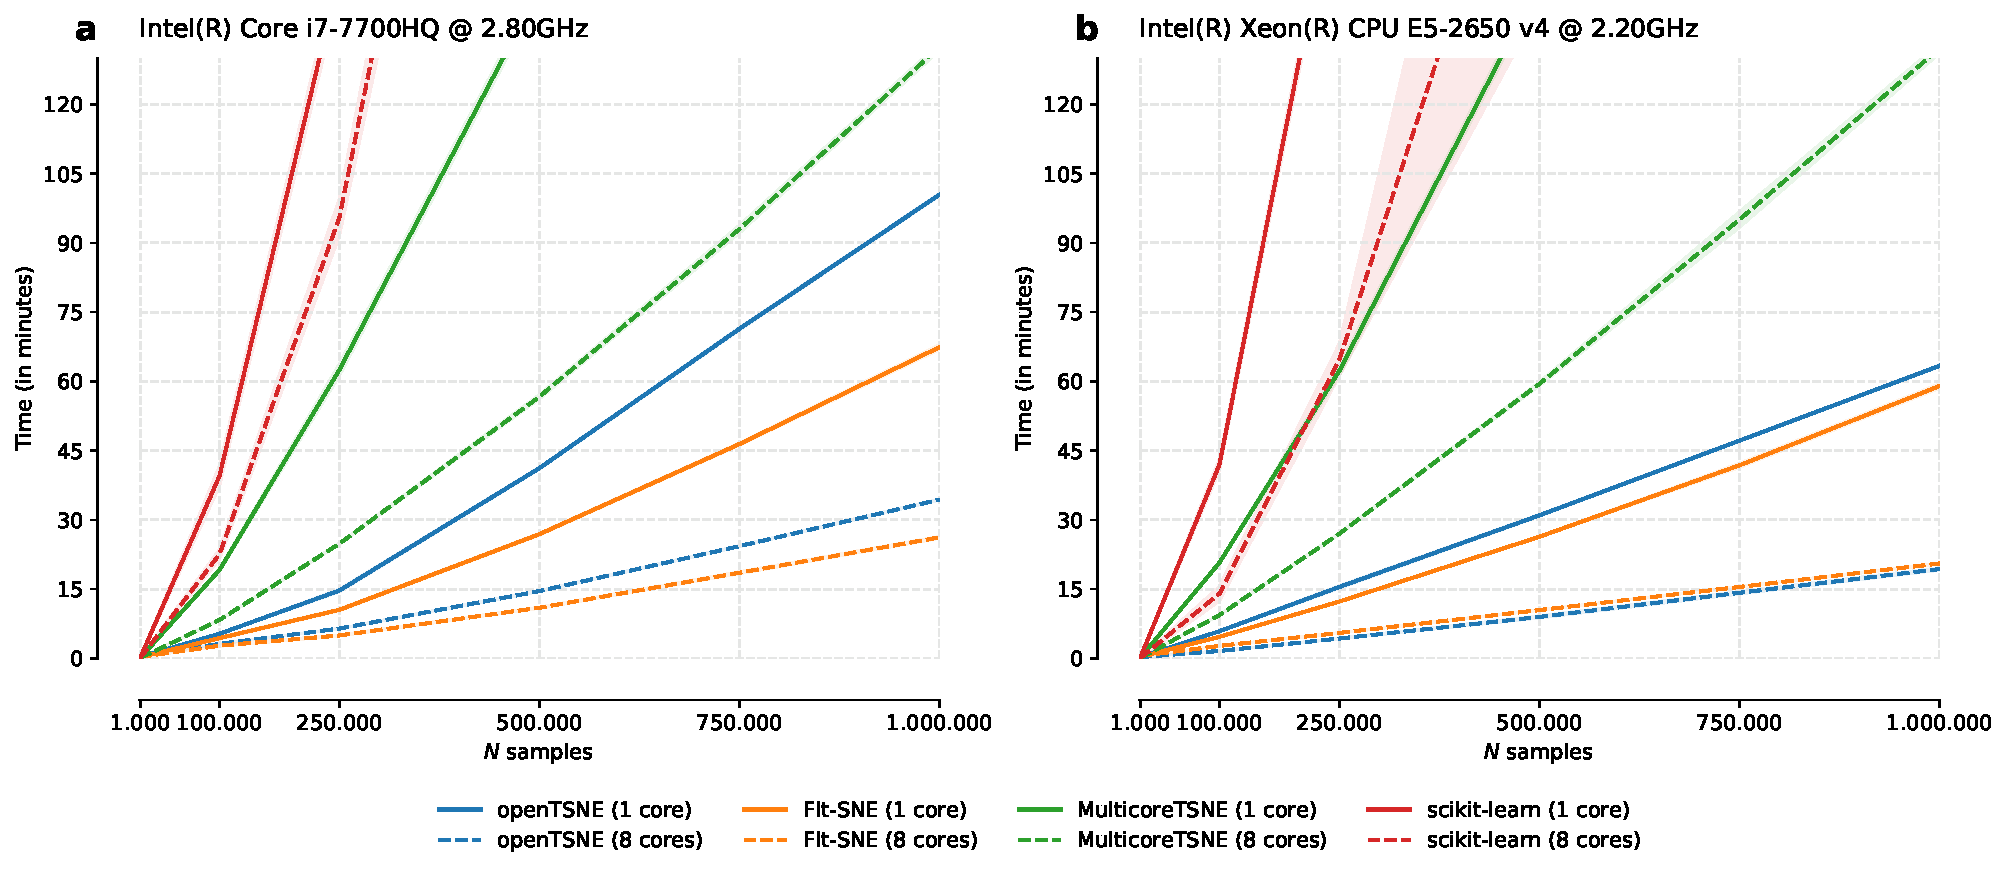
\includegraphics[width=\textwidth]{benchmarks}
  \caption{\label{fig:benchmarks}
  We benchmark \opentsne\ (v0.6.0) against three popular open-source
  implementations from \pkg{scikit-learn}~\citep{pedregosa2011scikit}
  (v0.23.1), \pkg{MulticoreTSNE}~\citep{Ulyanov2016} (v0.1), and
  \pkg{FIt-SNE}~\citep{linderman2019fast} (v1.1.0). Experiments were run on a
  consumer-grade Intel Core i7-7700HQ processor found in laptop computers, and
  on a server-grade Intel Xeon E5-2650. To generate benchmark data sets of
  different sizes, we subsampled data from the 10X Genomics 1.3 million mouse
  brain data set five times, resulting in five different data sets for each
  size. In total, we run each implementation on 30 different data sets. Notice
  that \opentsne\ scales similarly to \pkg{FIt-SNE}, as they both use the
  same interpolation-based approximation scheme, while \pkg{scikit-learn} and
  \pkg{MulticoreTSNE} utilize the Barnes-Hut approximation.
}
\end{figure*}

Benchmark results (Fig.~\ref{fig:benchmarks}) confirm that both \pkg{FIt-SNE}
and \opentsne\ scale better than their Barnes-Hut counterparts --
\pkg{scikit-learn} and \pkg{MulticoreTSNE}. While \opentsne's implementation
uses Python which incurs some runtime overhead compared to its C++ counterpart
\pkg{FIt-SNE}, the two libraries' speeds are surprisingly comparable. Modern
computer processors contain multiple cores, allowing us to use multi-threading,
which further reduces the gap between \opentsne\ and \pkg{FIt-SNE}. On the
server-grade processor, \opentsne\ is slightly faster than its pure C++
counterpart when utilizing multiple cores. \opentsne\ uses \pkg{numpy} for most
linear algebra operations, which may make better use of the Intel Math Kernel
Library (MKL), which is aggressively optimized on Intel(R) Xeon(R) processors.  

\opentsne\ provides a flexible API, allowing splitting up the
embedding-construction process into several parts, caching slow operations.
Running t-SNE optimization in stages enables users to quickly experiment with
different parameter settings and iterate on their final visualizations.

\subsection{Ease of Use}

Intuitive access and simple installation procedures almost universally correlate
with the widespread adoption of novel computational techniques. While the t-SNE
implementation from \pkg{scikit-learn} fits this requirement, the implementation
proves prohibitively slow for even moderately-sized data sets that span tens of
thousands of data records. Other C++ implementations such as \pkg{MulticoreTSNE}
and \pkg{FIt-SNE} exhibit better scaling in more massive data sets, but do not
provide precompiled binaries and require users to compile the software
themselves. This problem is critical, for instance, for users of the Windows
operating system, where the C++ compiler does not come with the system, making
the correct configuration of current t-SNE implementations cumbersome.

We designed \opentsne\ to be accessible to a broader audience. We provide
precompiled binaries for all major Python versions on all major platforms,
making the installation process as seamless as possible. One can install
\opentsne\ through the Python Package Index (\pkg{PyPI}) or \pkg{conda} from the
\pkg{conda-forge} channel, the two most widely adopted Python package managers.
\opentsne's interface is inspired by \pkg{scikit-learn}, which is well
established in the Python data science ecosystem. \opentsne\ implements
multi-threaded versions of both the Barnes-Hut and FIt-SNE approximation
schemes, enabling it to be applied to data sets containing millions of data
points. While the Python virtual machine inevitably introduces some performance
overhead, the runtime is comparable to its C++ counterpart -- \pkg{FIt-SNE}.
Finally, \opentsne\ is extensible. Its modular design enables researchers to
quickly experiment with different parameter settings and easily incorporate
custom components into the software. We provide a full feature list and
comparison to other popular t-SNE implementations in Table~\ref{tab:features}.


\begin{table}
\begin{center}\small
\newcommand*\rot{\rotatebox{45}}
\renewcommand{\arraystretch}{1.25}

\begin{tabular}{l c c c c c c c}
\toprule
\setlength\tabcolsep{6pt}
& \rot{\pkg{scikit-learn}} & \rot{\pkg{BHTSNE}} & \rot{\pkg{MulticoreTSNE}} & \rot{\pkg{FIt-SNE}} & \rot{\pkg{openTSNE}} \\

\toprule
\textbf{Ease of Installation}\\
Native Python installation & \checkmark & & & & \checkmark \\
\pkg{PyPI} package & \checkmark & & \checkmark & & \checkmark \\
\pkg{conda} package & \checkmark & & & & \checkmark \\

\hline
\textbf{Approximation Schemes}\\
Barnes-Hut ($\mathcal{O}(N \log N)$) & \checkmark & \checkmark & \checkmark & & \checkmark \\
FIt-SNE ($\mathcal{O}(N)$) & & & & \checkmark & \checkmark \\

\hline
\textbf{Advanced Features and Extensions}\\
Multiscale Gaussian kernels & & & & \checkmark & \checkmark \\
Fully-custom affinity kernels & & & & & \checkmark \\
Variable degrees of freedom & & & & \checkmark & \checkmark \\
Variable exaggeration & & & & \checkmark & \checkmark \\
Globally-consistent initialization & & & & \checkmark & \checkmark \\
Automatic learning rate & & & & \checkmark & \checkmark \\
Adding samples to embeddings & & & & & \checkmark \\
Callback system & & & & & \checkmark \\
Interactive optimization  & & & & & \checkmark \\

\hline
\textbf{Project Quality}\\
User documentation & \checkmark & & & & \checkmark \\
End-to-end usage examples & \checkmark & & & \checkmark & \checkmark \\
API reference & \checkmark & & & & \checkmark \\
Continuous integration & \checkmark & & \checkmark & & \checkmark \\
\bottomrule
\end{tabular}
\end{center}

\caption{\label{tab:features}
  We compare the features of \opentsne~(v0.6.0) to four popular open-source
  t-SNE implementations from \pkg{scikit-learn}~(v0.23.1),
  \pkg{BHTSNE}~(master), \pkg{MulticoreTSNE}~(v0.1), and
  \pkg{FIt-SNE}~(v1.1.0).
}
\end{table}


\section{Conclusion}
We introduce \opentsne, the most feature-complete, open-source, Python implementation of the widely popular t-SNE visualization algorithm. The library incorporates the latest developments to the t-SNE algorithm and makes them easily accessible through a familiar API. \opentsne\ implements efficient approximation schemes, making it suitable for the visualization of large data sets containing up to millions of data points. Finally, \opentsne\ is easy to install and comes with precompiled binaries available for all major platforms.


%% -- Optional special unnumbered sections -------------------------------------

\section*{Availability and Documentation}

\opentsne\ is distributed under the BSD-3-Clause License and its source code is
publicly available at \url{https://github.com/pavlin-policar/openTSNE}.
\opentsne\ can also be installed from \pkg{PyPI} and \pkg{conda-forge}.
End-to-end usage examples, documentation, and API reference are all available at
\url{https://opentsne.readthedocs.io}.

\section*{Computational details}

The results in this paper were obtained using \proglang{Python}~3.7.6 with the
\pkg{openTSNE}~v0.6.0 package. \opentsne\ has three direct dependencies:
\pkg{numpy}, \pkg{scipy}, and \pkg{scikit-learn}. In our experiments, we used
\pkg{numpy}~v1.18.1, \pkg{scipy}~v1.4.1. \pkg{scikit-learn}~v0.23.1. As these
packages include their own downstream dependencies, the full environment used to
produce the figures is included in the accompanying GitHub repository
\url{https://github.com/pavlin-policar/opentsne-paper}.

\section*{Acknowledgments}

We want to thank Dmitry Kobak for helpful discussions regarding t-SNE and
his contributions to the source code. We would also like to thank George
Linderman for his help with the FIt-SNE algorithm. This work was supported by
Slovenian Research Agency (P2-0209).


%% -- Bibliography -------------------------------------------------------------
%% - References need to be provided in a .bib BibTeX database.
%% - All references should be made with \cite, \citet, \citep, \citealp etc.
%%   (and never hard-coded). See the FAQ for details.
%% - JSS-specific markup (\proglang, \pkg, \code) should be used in the .bib.
%% - Titles in the .bib should be in title case.
%% - DOIs should be included where available.

\bibliography{references}

\end{document}
